\documentclass[aspectratio=169]{beamer}
\usepackage[utf8]{inputenc}
\usepackage[T1]{fontenc}
\usepackage{polski}
\usepackage{lmodern}
\usepackage{listings}
\usepackage{xcolor}
\usepackage{tikz}
\usetikzlibrary{shapes,arrows,positioning}

\usetheme{Madrid}
\usecolortheme{default}

\lstset{
    language=Python,
    basicstyle=\ttfamily\footnotesize,
    keywordstyle=\color{blue},
    stringstyle=\color{red},
    commentstyle=\color{gray},
    showstringspaces=false,
    breaklines=true,
    frame=single,
    numbers=left,
    numberstyle=\tiny\color{gray},
    literate={@}{{@}}1 {\#}{{\#}}1
}

\setbeamertemplate{navigation symbols}{}
\setbeamertemplate{footline}{}

\title{Bridge (Most)}
\subtitle{czyli jak nie utopić się w eksplozji klas}
\author{Wzorce projektowe -- laboratorium}
\date{21 listopada 2025}

\begin{document}

\frame{\titlepage}

\begin{frame}{Wyobraź sobie...}
\begin{center}
\Large
Piszesz symulator botów internetowych (w celach edukacyjnych!).
\end{center}

\pause

\vspace{0.5cm}

Masz typy botów:
\begin{itemize}
    \item \textbf{Troll} -- prowokuje kłótnie
    \pause
    \item \textbf{Spammer} -- promuje krypto i ,,okazje''
    \pause
    \item \textbf{Conspiracist} -- wszędzie widzi spiski
    \pause
    \item \textbf{FakeNews} -- szerzy dezinformację
\end{itemize}

\pause

\vspace{0.3cm}

I platformy:
\begin{itemize}
    \item Twitter, Facebook, LinkedIn, TikTok
\end{itemize}

\pause

\vspace{0.3cm}

\begin{center}
\textbf{4 boty x 4 platformy = 16 klas?!} To się nie skończy dobrze...
\end{center}
\end{frame}

\begin{frame}[fragile]{Bez Bridge -- eksplozja klas}
\begin{lstlisting}[basicstyle=\ttfamily\tiny]
class TrollTwitterBot:
    def post(self, topic):
        return f"@everyone {topic}?! HAHA serio w to wierzysz? ratio"

class TrollFacebookBot:
    def post(self, topic):
        return f"{topic}... ciekawe... TYLKO IDIOCI w to wierza!!!"

class TrollLinkedInBot:
    def post(self, topic):
        return f"Unpopular opinion: {topic} is WRONG. Agree?"

class TrollTikTokBot:
    def post(self, topic):
        return f"pov: ktos mowi ze {topic} ma sens XDDD"

class SpammerTwitterBot:
    def post(self, topic):
        return f"NEW {topic} COIN! 1000x guaranteed! Link in bio!"

class SpammerFacebookBot:
    def post(self, topic):
        return f"Moja kuzynka zarobila 5000 na {topic}!!! Szczegoly w DM"

# ... i tak dalej dla 16 klas!
\end{lstlisting}
\end{frame}

\begin{frame}{Problem}
\begin{itemize}
    \item Masz \textbf{dwa niezależne wymiary}: typ bota i platforma
    \item Każda kombinacja = \textbf{osobna klasa}
    \item 4 boty x 4 platformy = \textbf{16 klas}
    \item Dodajesz Mastodon? \textbf{+4 nowe klasy}
    \item Dodajesz nowego bota? \textbf{+4 nowe klasy}
    \item 10 botów x 10 platform = \textbf{100 klas!}
\end{itemize}

\vspace{0.5cm}

\begin{center}
\Large
To się nazywa \textbf{eksplozja klas}. \\
\vspace{0.3cm}
\normalsize
I to jest właśnie problem, który rozwiązuje \textbf{Bridge}.
\end{center}
\end{frame}

\begin{frame}{Wzorzec Bridge -- idea}
\begin{center}
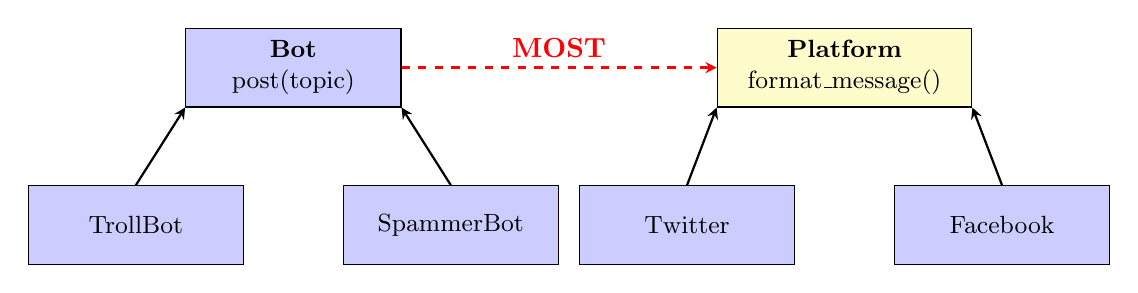
\begin{tikzpicture}[
    class/.style={rectangle, draw=black, fill=blue!20, text width=2.5cm, text centered, minimum height=1cm, font=\small},
    interface/.style={rectangle, draw=black, fill=yellow!20, text width=3cm, text centered, minimum height=1cm, font=\small},
    arrow/.style={->, >=stealth, thick},
    bridge/.style={->, >=stealth, thick, dashed, red}
]
    % Lewa strona - Abstrakcja
    \node[class] (bot) at (0, 2) {\textbf{Bot}\\post(topic)};
    \node[class] (troll) at (-2, 0) {TrollBot};
    \node[class] (spammer) at (2, 0) {SpammerBot};
    
    % Prawa strona - Implementacja
    \node[interface] (platform) at (7, 2) {\textbf{Platform}\\format\_message()};
    \node[class] (twitter) at (5, 0) {Twitter};
    \node[class] (facebook) at (9, 0) {Facebook};
    
    % Strzalki dziedziczenia
    \draw[arrow] (troll.north) -- (bot.south west);
    \draw[arrow] (spammer.north) -- (bot.south east);
    \draw[arrow] (twitter.north) -- (platform.south west);
    \draw[arrow] (facebook.north) -- (platform.south east);
    
    % Most!
    \draw[bridge] (bot.east) -- node[above] {\textbf{MOST}} (platform.west);
\end{tikzpicture}
\end{center}

\vspace{0.5cm}

\textbf{Idea:} Rozdziel abstrakcję (typ bota) od implementacji (platforma). \\
Połącz je \textit{mostem} -- referencja zamiast dziedziczenia!

\vspace{0.3cm}

\textbf{4 + 4 = 8 klas} zamiast \textbf{4 x 4 = 16 klas}
\end{frame}

\begin{frame}[fragile]{Z Bridge -- elegancki kod}
\begin{lstlisting}[basicstyle=\ttfamily\tiny]
from abc import ABC, abstractmethod

# Implementacja (platforma)
class Platform(ABC):
    @abstractmethod
    def format_message(self, message: str) -> str:
        pass

class Twitter(Platform):
    def format_message(self, message: str) -> str:
        return f"{message[:280]} #viral"

class LinkedIn(Platform):
    def format_message(self, message: str) -> str:
        return f"{message}\n\nAgree? Let's discuss. #OpenToWork"

# Abstrakcja (bot)
class Bot(ABC):
    def __init__(self, platform: Platform):
        self.platform = platform  # <-- MOST!
    
    @abstractmethod
    def generate_content(self, topic: str) -> str:
        pass
    
    def post(self, topic: str) -> str:
        content = self.generate_content(topic)
        return self.platform.format_message(content)  # <-- Delegacja!
\end{lstlisting}
\end{frame}

\begin{frame}[fragile]{Z Bridge -- konkretne boty}
\begin{lstlisting}
class TrollBot(Bot):
    def generate_content(self, topic: str) -> str:
        return f"Serio wierzysz w {topic}? HAHA!"

class SpammerBot(Bot):
    def generate_content(self, topic: str) -> str:
        return f"NOWY {topic} COIN! 1000x gwarantowane!"

# Uzycie - kompozycja zamiast 16 klas!
troll_twitter = TrollBot(Twitter())
troll_linkedin = TrollBot(LinkedIn())
spammer_twitter = SpammerBot(Twitter())

print(troll_twitter.post("AI"))
# "Serio wierzysz w AI? HAHA! #viral"

print(troll_linkedin.post("AI"))
# "Serio wierzysz w AI? HAHA!\n\nAgree? Let's discuss. #OpenToWork"
\end{lstlisting}
\end{frame}

\begin{frame}{Co tu się dzieje? -- Krok po kroku}
\begin{center}
\Large
\textbf{1. Rozdzielamy dwa wymiary}
\end{center}

\vspace{0.5cm}

\begin{columns}
\begin{column}{0.48\textwidth}
\textbf{Abstrakcja (CO robi):}
\begin{itemize}
    \item Bot
    \item TrollBot
    \item SpammerBot
    \item ConspiracistBot
    \item FakeNewsBot
\end{itemize}
\end{column}
\begin{column}{0.48\textwidth}
\textbf{Implementacja (JAK wygląda):}
\begin{itemize}
    \item Platform
    \item Twitter
    \item Facebook
    \item LinkedIn
    \item TikTok
\end{itemize}
\end{column}
\end{columns}

\vspace{0.5cm}

\begin{center}
Każdy wymiar może się zmieniać \textbf{niezależnie}!
\end{center}
\end{frame}

\begin{frame}[fragile]{Co tu się dzieje? -- Most w akcji}
\begin{center}
\Large
\textbf{2. Łączymy mostem (kompozycja)}
\end{center}

\vspace{0.5cm}

\begin{lstlisting}[language=Python, basicstyle=\ttfamily\small]
class Bot(ABC):
    def __init__(self, platform: Platform):
        self.platform = platform  # <-- To jest MOST!
\end{lstlisting}

\vspace{0.5cm}

\begin{itemize}
    \item Bot \textbf{ma} platformę (kompozycja)
    \item Bot \textbf{nie jest} platformą (brak dziedziczenia!)
    \item Można zmienić platformę w runtime!
\end{itemize}

\vspace{0.3cm}

\begin{lstlisting}[language=Python, basicstyle=\ttfamily\small]
troll = TrollBot(Twitter())
troll.platform = LinkedIn()  # Zmiana platformy!
\end{lstlisting}
\end{frame}

\begin{frame}[fragile]{Porównanie: Przed i Po}
\begin{columns}
\begin{column}{0.48\textwidth}
\textbf{Przed (eksplozja klas):}
\begin{lstlisting}[basicstyle=\ttfamily\tiny]
TrollTwitterBot
TrollFacebookBot
TrollLinkedInBot
TrollTikTokBot
SpammerTwitterBot
SpammerFacebookBot
SpammerLinkedInBot
SpammerTikTokBot
ConspiracistTwitterBot
ConspiracistFacebookBot
# ... 16 klas!
\end{lstlisting}

\textcolor{red}{[X]} 16 klas do utrzymania\\
\textcolor{red}{[X]} Nowa platforma = +4 klasy\\
\textcolor{red}{[X]} Kod się powtarza
\end{column}
\begin{column}{0.48\textwidth}
\textbf{Po (Bridge):}
\begin{lstlisting}[basicstyle=\ttfamily\tiny]
# Boty (4)
Bot (abstract)
TrollBot
SpammerBot
ConspiracistBot
FakeNewsBot

# Platformy (4)
Platform (abstract)
Twitter
Facebook
LinkedIn
TikTok
\end{lstlisting}

\textcolor{green}{[OK]} 8 klas zamiast 16\\
\textcolor{green}{[OK]} Nowa platforma = +1 klasa\\
\textcolor{green}{[OK]} Brak powtórzeń
\end{column}
\end{columns}
\end{frame}

\begin{frame}{Kiedy używać Bridge?}
\begin{itemize}
    \item Masz \textbf{dwa niezależne wymiary} zmienności
    \item Chcesz uniknąć \textbf{eksplozji klas}
    \item Abstrakcja i implementacja powinny móc się zmieniać \textbf{niezależnie}
    \item Chcesz móc \textbf{zmieniać implementację w runtime}
\end{itemize}

\vspace{0.5cm}

\textbf{Przykłady z życia:}
\begin{itemize}
    \item Urządzenie (pilot, telefon) + System (TV, klimatyzacja)
    \item Kształt (koło, kwadrat) + Kolor (czerwony, niebieski)
    \item Widok (lista, siatka) + Źródło danych (API, baza, plik)
\end{itemize}

\vspace{0.5cm}

\textbf{Trade-off:} Więcej abstrakcji, ale \textit{znacznie} mniej klas przy wielu kombinacjach.
\end{frame}

\begin{frame}{Dzisiaj na zajęciach}
\begin{enumerate}
    \item Dostaniecie kod symulatora botów (z eksplozją klas): \\
    \texttt{https://github.com/refactor-or-die/lab04-totally-not-a-bot}
    \item W parach zrefaktoryzujecie go używając wzorca Bridge
    \item Rozdzielicie boty od platform
\end{enumerate}

\vspace{1cm}

\begin{center}
\Large
\textbf{Pytania?} \\
\vspace{0.5cm}
\normalsize
Jeśli nie -- to \texttt{git clone} i budujemy mosty! \\
\end{center}
\end{frame}

\end{document}
